%!TEX program = xelatex
% 完整编译: xelatex -> biber/bibtex -> xelatex -> xelatex
\documentclass[lang=cn,11pt,a4paper]{elegantpaper}

\title{fraction.h文档说明}
\author{Haochen Huang}

\version{2.02test}
\date{\zhtoday}


% 本文档命令
\usepackage{array}

\begin{document}

\maketitle
\tableofcontents

\begin{abstract}
本文为basilisk的头文件fraction.h的说明文档,本文档中大量函数引用自geometry.h,其具体实现方法请移步geometry.h说明文档\par
2.02更新:根据反馈更新了大量的注释,同时新增fraction refine等函数的理论说明
\end{abstract}


\section{文件中主要函数及目的}
本头文件中所提供的绝大部分函数都是为了服务VOF方法,其构建的大量函数将在vof.h中被引用,针对两相不同界面进行处理操作,其具体功能分别是:
\begin{itemize}
    \item fraction refine函数\ref{sec:fracrefine}:用于在树状网格结构中对子单元的界面法向量$\mathbf{n}$,界面内体积分数$c$,以及界面常数$\alpha$进行构建
    \item fraction函数\ref{sec:fraction}:本头文件的核心内容,其主要功能是根据用户提供的Level-set函数直接构建两相界面,在既定网格上合理分配相关的边界内体积分数,单位法向量等。
    \item facet normal函数\ref{sec:facetnorm}:根据输入单元的体积分数$c$或者是单元面表面体积分数$s$对界面法向量进行计算。
    \item reconstruction函数\ref{sec:reconstruction}:利用myc函数,输入$c$返回单元的法向量与界面参数$\alpha$
    \item output facets函数\ref{sec:outputfacets}:根据输出的数据结构返回界面与单位边界交点,供后期处理时对边界进行描绘
    \item interface area函数\ref{sec:interfacial}:根据界面信息返回界面面积或长度。
\end{itemize}
\section{fraction refine函数}\label{sec:fracrefine}
本函数目的在于针对树状结构网格,重新构建相应的子网格边界定义,相关预置设置在本节中也有所体现。
\subsection{理论原理}
本节代码中重要的理论原理请移步myc.h说明文档以及geometry.h说明文档。
\subsection{代码实现}
\begin{minted}[mathescape=true,breaklines]{lexer.py:DiffLexer -x}
#include "geometry.h"
#if dimension == 1
coord mycs (Point point, scalar c) {
  coord n = {1.};
  return n;
}
#elif dimension == 2
# include "myc2d.h"
#else // dimension == 3
# include "myc.h"
#endif

/**
By default the interface normal is computed using the MYC
approximation. This can be overloaded by redefining this macro. */

#ifndef interface_normal
# define interface_normal(point, c) mycs (point, c)//计算两相界面法向量,此处的mycs函数是从myc.h中抽取出来的
#endif
\end{minted}
相关预设值工作在此结束,需要注意的是代码根据3D或2D情况,从myc.h以及myc2d.h中抽取相关函数对定义为法向量拟合函数。接下来为树状网格边界重构的相关代码。
\begin{minted}[mathescape=true,breaklines]{lexer.py:DiffLexer -x}
/**
## Coarsening and refinement of a volume fraction field 

On trees, we need to define how to coarsen (i.e. "restrict") or
refine (i.e. "prolongate") interface definitions (see [geometry.h]()
for a basic explanation of how interfaces are defined). */
//说明:树形网格中,网格内体积分数及截距的重构

#if TREE

void fraction_refine (Point point, scalar c)
{
  
  /**
  If the parent cell is empty or full, we just use the same value for
  the fine cell. */

  double cc = c[];
  if (cc <= 0. || cc >= 1.)
    foreach_child()
      c[] = cc;
  else {

    /**
    Otherwise, we reconstruct the interface in the parent cell. */

    coord n = mycs (point, c);
    double alpha = plane_alpha (cc, n);

    /**
    And compute the volume fraction in the quadrant of the coarse cell
    matching the fine cells. We use symmetries to simplify the
    combinations. */

    foreach_child() {
      static const coord a = {0.,0.,0.}, b = {.5,.5,.5};//从3D角度讲就是选取第一象限中的子单元
      coord nc;
      foreach_dimension()
         nc.x = child.x*n.x;//转换坐标,将各个象限的子单元通过坐标转换的方式让其存在于第一象限
      c[] = rectangle_fraction (nc, alpha, a, b);//本函数请详细geometry.h说明文档,其作用是计算通过坐标a,b定义的单元中的方形区域的体积分数
    }
  }
}

/**
Finally, we also need to prolongate the reconstructed value of
$\alpha$. This is done with the simple formula below. We add an
attribute so that we can access the normal from the refinement
function. */

attribute {
  vector n;
}

static void alpha_refine (Point point, scalar alpha)
{
  vector n = alpha.n;
  double alphac = 2.*alpha[];
  coord m;
  foreach_dimension()
    m.x = n.x[];
  foreach_child() {
    alpha[] = alphac;
    foreach_dimension()
      alpha[] -= child.x*m.x/2.;
  }
}

#endif // TREE
\end{minted}
fraction refine函数中的rectangle fraction函数的调用是其重点,其最终目的是通过确定第一象限中的子单元(其中两点的坐标为$a=(0,0,0),b=(\frac{1}{2},\frac{1}{2},\frac{1}{2})$),通过拟合的法向量,求取相应的体积分数。依旧以2D单元为例:\par
\begin{figure}[htbp]
    \centering
    \begin{center}
    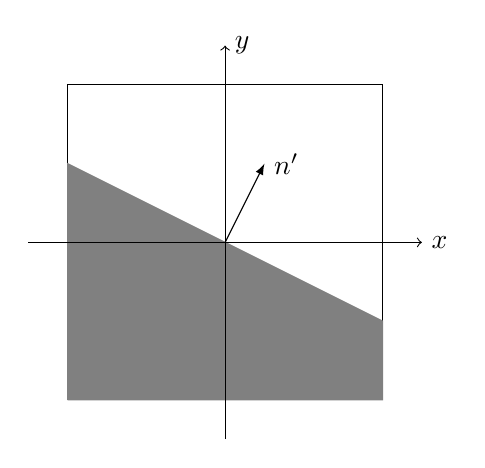
\begin{tikzpicture}[scale=1]
    \draw (-2,0)--(2,0)--(2,4)--(-2,4)--(-2,0);
    \filldraw[gray] (-2,0)--(-2,3)--(2,1)--(2,0)--(-2,0);
    \draw[->] (0,-0.5)--(0,4.5) node[anchor=west]{$y$};
    \draw[->] (-2.5,2.0)--(2.5,2.0) node[anchor=west]{$x$};
    \draw[-latex](0,2)--(0.5,3) node[anchor=west]{$n'$};
    \end{tikzpicture}
    \end{center}
    \caption{坐标变换示例}
    \label{fig:pianyi1}
\end{figure}
该单元具有四个子单元,代码中$child.x$即为各个子单元的指代参数值为$1,-1$,上图中,位于第三象限子单元的相关参数为$child.x=-1,child.y=-1$,如果想利用坐标变换将第三象限转换至第一象限的坐标变换为:
\begin{equation}
    \left\{ 
    \begin{array}{cc}
    x'=&x\times -1\\
    y'=&y\times -1
    \end{array}
    \right.
\end{equation}
综上对任意子单元,进行坐标变换都有
\begin{equation}
    n'=(child.x\times n_x,child.y\times n_y)
\end{equation}
而对于alpha refine函数情况相对复杂,该函数目的是将子单元变为单一单元,并将坐标轴移至子单元中心,坐标单位长度以子单元边长为准,为了简便,以三象限单元为例:
\begin{figure}[htbp]
    \centering
    \begin{center}
    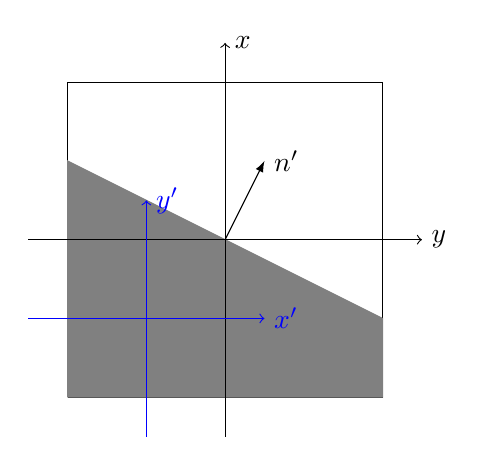
\begin{tikzpicture}[scale=1]
    \draw (-2,0)--(2,0)--(2,4)--(-2,4)--(-2,0);
    \filldraw[gray] (-2,0)--(-2,3)--(2,1)--(2,0)--(-2,0);
    \draw[->] (0,-0.5)--(0,4.5) node[anchor=west]{$x$};
    \draw[->] (-2.5,2.0)--(2.5,2.0) node[anchor=west]{$y$};
    \draw[blue,->] (-2.5,1)--(0.5,1) node[anchor=west]{$x'$};
    \draw[blue,->] (-1,-0.5)--(-1,2.5) node[anchor=west]{$y'$};
    \draw[-latex](0,2)--(0.5,3) node[anchor=west]{$n'$};
    \end{tikzpicture}
    \end{center}
    \caption{坐标变换示例}
    \label{fig:pianyi1}
\end{figure}
在坐标变换是首先要进行单位变化,由于在本单元内单元长度为1,而以子单元为坐标时,子单元长度变为1,需要首先对单元长度进行变换,再根据变换后的原点位置对坐标轴进行移动,综上有:
\begin{equation}
    \alpha'=2\alpha-\frac{1}{2}(n_x\times child.x+n_y\times child.y)
\end{equation}
\section{fraction函数}\label{sec:fraction}
本函数的目的在于根据给定输入的Level-set函数直接确定不同相边界。
\subsection{理论原理}
Level-set函数意在使用函数$\Phi(\mathbf{x},t)$对边界内$\Omega$进行表达,针对空间中坐标为$\mathbf{x_0}$,在时间$t= t_0$的某一点,若
\begin{gather}
    \Phi(\mathbf{x_0},t_0)>0 \quad for \quad \mathbf{x_0}\in\Omega\nonumber\\
    \Phi(\mathbf{x_0},t_0)<0 \quad for \quad \mathbf{x_0}\notin\Omega\\
    \Phi(\mathbf{x_0},t_0)=0 \quad for \quad \mathbf{x_0}\in\partial\Omega\nonumber
\end{gather}
\begin{figure}[H]
    \centering
    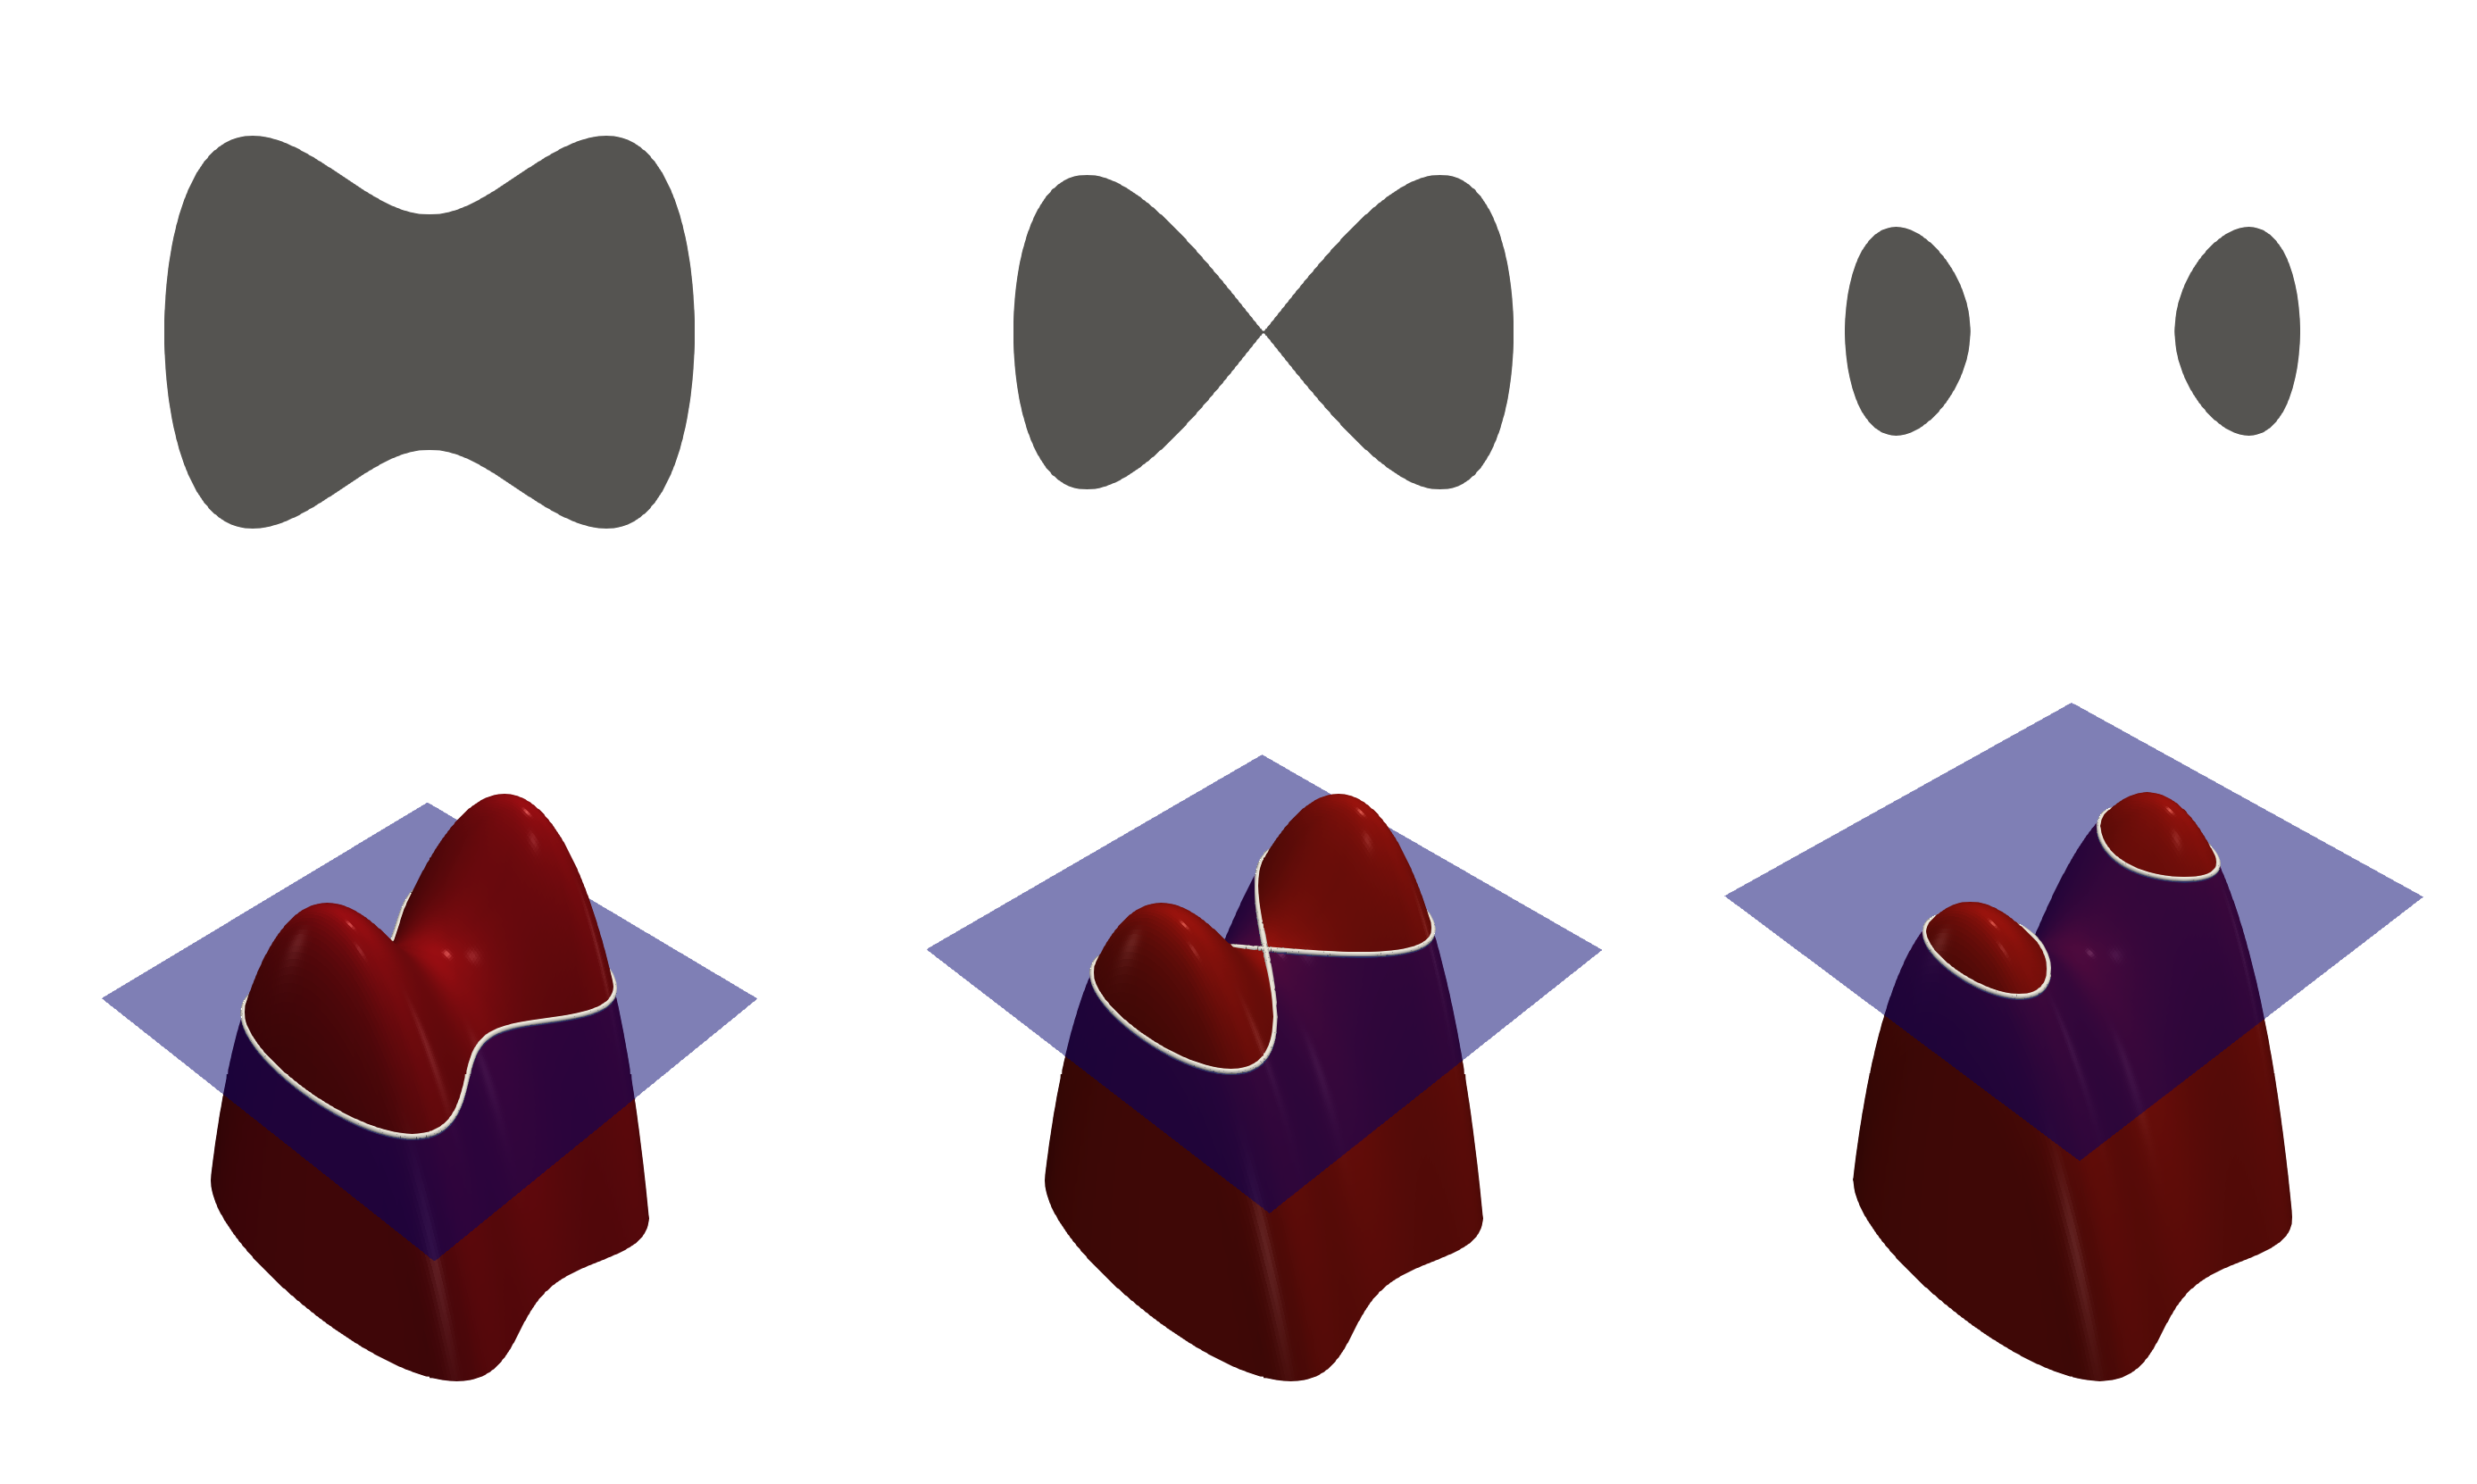
\includegraphics[scale = 0.15]{Level_set_method.png}
    \caption{本图片引自\cite{NBS_2021}}
    \label{levelset}
\end{figure}
以2D为例,我们可以利用该函数,对空间中每一选定点在某一时刻进行赋值;针对所画网格的节点(注意是每一网格的四个拐角点,而并非网格中心)进行上述操作有:
\begin{figure}[H]
\begin{center}
    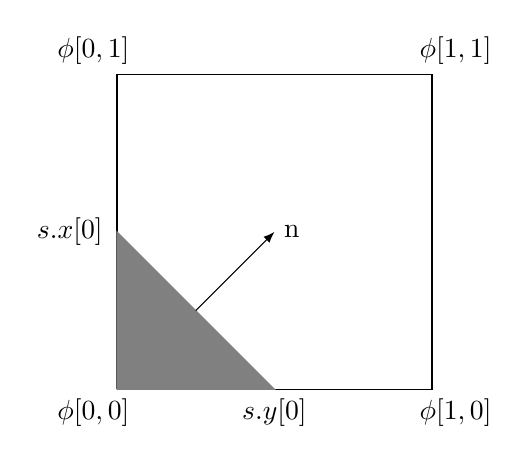
\begin{tikzpicture}[scale=1]
    \draw (-2,0)--(2,0)--(2,4)--(-2,4)--(-2,0);
    \node(a) at (-2.3,-0.3) {$\phi[0,0]$};
    \node(b) at (-2.3,4.3) {$\phi[0,1]$};
    \node(c) at (2.3,-0.3) {$\phi[1,0]$};
    \node(d) at (2.3,4.3) {$\phi[1,1]$};
    \node(e) at (0,-0.3) {$s.y[0]$};
    \node(f) at (-2.6,2.0) {$s.x[0]$};
    \filldraw[gray] (-2,0)--(-2,2)--(0,0)--(-2,0);
    \draw[-latex](-1,1)--(0,2) node[anchor=west]{n};
    \end{tikzpicture}
\end{center}
\caption{2D示例单元}
\end{figure}
通过对节点的插值,我们可以得到单元边界面上的面积分数,并将其存储在face
vector型数据中。\par
我们借此来计算单元中的法向量,首先在图中单元边界内部对法向量$\mathbf{n}$进行积分有:
\begin{equation}
    \oint_{\partial \Omega}\mathbf{n}dl = 0
\end{equation}
我们取$x$分量有:
\begin{equation}
    -s_x[]+\int_{\phi = 0}n_xdl = 0
\end{equation}
令
\begin{equation}
    \bar{\mathbf{n}} = \int_{\phi = 0}\mathbf{n}dl
\end{equation}
则有$\bar{n_x} = s_x[] - s_x[1]$,而$\bar{\mathbf{n}}$的模长为
\begin{equation}
    \lvert \bar{\mathbf{n}} \rvert = \int_{\phi=0}dl
\end{equation}
又因为我们假设边界均为直线段,是故可以直接通过$n_x = \frac{\bar{n_x}}{\lvert \bar{\mathbf{n}} \rvert}$求出相应的精准法向量。\par
自此我们可以使用geometry.h中的函数对边界上网格进行划分。
\subsection{代码实现}

\begin{minted}[mathescape=true,breaklines]{lexer.py:DiffLexer -x}
struct Fractions {
  vertex scalar Phi; // compulsory
  scalar c;          // compulsory
  face vector s;     // optional
  double val;        // optional (default zero)
};
//定义Fraction型数据结构,将$\phi$定义为在每个角节点上的数据,其中val是用于控制边界表示的参数,一般取默认值0

trace
void fractions (struct Fractions a)
{
  vertex scalar Phi = a.Phi;
  scalar c = a.c;
  face vector s = automatic (a.s);
  double val = a.val;
  #if dimension == 3
  vector p[];
#else // dimension == 2
  vector p;
  p.x = s.y; p.y = s.x;
#endif

  foreach_edge() {
//首先针对每一条边进行判断,若该单元边界的两顶点的Level-set函数值正负不一样,则代表着这条边处在两相之间,需要对其边界体积分数进行计算。
    if ((Phi[] - val)*(Phi[1] - val) < 0.) {
      p.x[] = (Phi[] - val)/(Phi[] - Phi[1]);
      if (Phi[] < val)
        p.x[] = 1. - p.x[];
    }

    else
      p.x[] = (Phi[] > val || Phi[1] > val);
  }
  
#if dimension == 3//如果为3D情况则需要三次变换,分别是从边界体积分数到面体积分数,再到3维单元的体积分数
  scalar s_x = s.x, s_y = s.y, s_z = s.z;
  foreach_face(z,x,y)
#else // dimension == 2
  boundary_flux ({s});
  scalar s_z = c;//当为2维情况时为了表达简便,将原本存放z方向面体积分数的数据储存留给整体的体积分数
  foreach()
#endif
  {
    coord n;
    double nn = 0.;
    foreach_dimension(2) {
      n.x = p.y[] - p.y[1];
      nn += fabs(n.x);//注意此处所谓的向量单位化并不是非常单纯的令该法向量的模长为1,而是使得改变之后的$n_x+n_y = 1$
    }
    if (nn == 0.)
      s_z[] = p.x[];
    else {
      foreach_dimension(2)
        n.x /= nn;

      double alpha = 0., ni = 0.;
      for (int i = 0; i <= 1; i++)
        foreach_dimension(2)
          if (p.x[0,i] > 0. && p.x[0,i] < 1.) {
            double a = sign(Phi[0,i] - val)*(p.x[0,i] - 0.5);
            alpha += n.x*a + n.y*(i - 0.5);
            ni++;
      }
      //此处两处-0.5其实质上为从单元中心移到网格左下角,具体请见geometry.h。值得一提的是由于方程写作$n_xx+n_yy=\alpha$故$n_x,n_y$的取值会影响$alpha$但在相应算法中并不影响体积分数$c$
      if (ni == 0)
    s_z[] = max (p.x[], p.y[]);
      else if (ni != 4)
    s_z[] = line_area (n.x, n.y, alpha/ni);//此处将累加\alpha平均,通过geometry.h文件中函数求取该平面体积分数
      else {
#if dimension == 3
    s_z[] = (p.x[] + p.x[0,1] + p.y[] + p.y[1] > 2.);
#else
    s_z[] = 0.;
#endif
      }
    }
  }
  
#if dimension == 3
  boundary_flux ({s});
  foreach() {

    coord n;
    double nn = 0.;
    foreach_dimension(3) {
      n.x = s.x[] - s.x[1];
      nn += fabs(n.x);
    }
    if (nn == 0.)
      c[] = s.x[];
    else {
      foreach_dimension(3)
    n.x /= nn;
      
      double alpha = 0., ni = 0.;
      for (int i = 0; i <= 1; i++)
    for (int j = 0; j <= 1; j++)
      foreach_dimension(3)
        if (p.x[0,i,j] > 0. && p.x[0,i,j] < 1.) {
          double a = sign(Phi[0,i,j] - val)*(p.x[0,i,j] - 0.5);
          alpha += n.x*a + n.y*(i - 0.5) + n.z*(j - 0.5);
          ni++;
        }

      if (ni == 0)
    c[] = s.x[];
      else if (ni < 3 || ni > 6)
    c[] = 0.; 
    c[] = plane_volume (n, alpha/ni);
    }
  }
#endif // dimension == 3
  

  boundary ({c});
}

#define fraction(f,func) do {            \
    vertex scalar phi[];            \
    foreach_vertex()                \
      phi[] = func;                \ //在此类宏中,可以带入自定义的函数表达式,在每一个单元格的节点上带入func进行操作赋值,由该指令直接调动上文中的fractions函数,从而实现对处于边界上网格中边界的布置
    boundary ({phi});               \
    fractions (phi, f);             \
  } while(0)
\end{minted}
单行代码展示\mintinline{lexer.py:DiffLexer -x}{double un = dt*uf.x[]/(fm.x[]*Delta + SEPS), s = sign(un);} 
\section{facet normal}\label{sec:facetnorm}
本函数由目的在于计算单元法向量,输入量有两种形式,分别是单元体积分数$c$,或者单元边界面积分数$s$,通过不同方式进行计算。
\subsection{理论原理}
使用体积分数计算法向量的算法详细的在myc.h说明文件中进行了阐释,而利用单元表面面积分数计算法向量的原理则在上一节(即fraction函数)中充分阐述过了。
\subsection{代码实现}
\begin{minted}[mathescape=true,breaklines]{lexer.py:DiffLexer -x}
coord facet_normal (Point point, scalar c, face vector s)
{
  if (s.x.i >= 0) { // compute normal from face fractions
    coord n;
    double nn = 0.;
    foreach_dimension() {
      n.x = s.x[] - s.x[1];
      nn += fabs(n.x);
    }
    if (nn > 0.)
      foreach_dimension()
    n.x /= nn;
    else
      foreach_dimension()
    n.x = 1./dimension;
    return n;
  }
  return interface_normal (point, c);//如果没有单元表面面积分数,则调用myc中的函数直接利用周围单元的体积分数对法向量进行插值
}
\end{minted}
\section{reconstruction函数}\label{sec:reconstruction}
利用调用的myc函数,直接由目标单元的体积分数得到相应的法向量以及界面参数$\alpha$,相关理论请移步myc.h说明文件。
\subsection{代码实现}
\begin{minted}[mathescape=true,breaklines]{lexer.py:DiffLexer -x}
/**
### Interface reconstruction 

The reconstruction function takes a volume fraction field `c` and
returns the corresponding normal vector field `n` and intercept field
$\alpha$. */


trace
void reconstruction (const scalar c, vector n, scalar alpha)
{
  foreach() {

    /**
    If the cell is empty or full, we set $\mathbf{n}$ and $\alpha$ only to
    avoid using uninitialised values in `alpha_refine()`. */

    if (c[] <= 0. || c[] >= 1.) {
      alpha[] = 0.;
      foreach_dimension()
        n.x[] = 0.;
    }
    else {

      /**
      Otherwise, we compute the interface normal using the
      Mixed-Youngs-Centered scheme, copy the result into the normal field
      and compute the intercept $\alpha$ using our predefined function. */

      coord m = interface_normal (point, c);
      foreach_dimension()
    n.x[] = m.x;
      alpha[] = plane_alpha (c[], m);
    }
  }

#if TREE

  /**
  On a tree grid, for the normal to the interface, we don't use
  any interpolation from coarse to fine i.e. we use straight
  "injection". */
  //在树状网格结构中,我们直接使用网格设定中自带的函数对网格细化改进进行定义

  foreach_dimension()
    n.x.refine = n.x.prolongation = refine_injection;//refine injection为一内联函数,其定义在于将取得的scalar型变量赋予本单元内所有的子单元

  /**
  We set our refinement function for *alpha*. */

  alpha.n = n;
  alpha.refine = alpha.prolongation = alpha_refine;
#endif
}
\end{minted}
\section{output facets函数}\label{sec:outputfacets}
用于向指定文件输出单元与界面的交点坐标,从而在后处理中可以用直线将相关坐标点相连后得到两相边界情况。相应的具体原理也请参看geometry.h文件说明。
\subsection{代码实现}
\begin{minted}[mathescape=true,breaklines]{lexer.py:DiffLexer -x}
struct OutputFacets {
  scalar c;
  FILE * fp;     // optional: default is stdout
  face vector s; // optional: default is none
};

trace
void output_facets (struct OutputFacets p)
{
  scalar c = p.c;
  face vector s = p.s;
  if (!p.fp) p.fp = stdout;//如果并没有定义相关输出数据储存位置,则默认定义为标准输出
  if (!s.x.i) s.x.i = -1;//如果没有输入单元表面面积分数,则将其定义为负数

  foreach()
    if (c[] > 1e-6 && c[] < 1. - 1e-6) {
      coord n = facet_normal (point, c, s);
      double alpha = plane_alpha (c[], n);//利用geometry.h中的相关函数进行边界函数求解
#if dimension == 2      
      coord segment[2];
      if (facets (n, alpha, segment) == 2)
         fprintf (p.fp, "%g %g\n%g %g\n\n", 
         x + segment[0].x*Delta, y + segment[0].y*Delta, 
         x + segment[1].x*Delta, y + segment[1].y*Delta);//如果为2维情况,且确定单元被界面分割,则使用geometry中facet函数定义计算交点坐标,并将其输出至stdout中
#else // dimension == 3 3维同理
      coord v[12];
      int m = facets (n, alpha, v, 1.);
      for (int i = 0; i < m; i++)
         fprintf (p.fp, "%g %g %g\n",
         x + v[i].x*Delta, y + v[i].y*Delta, z + v[i].z*Delta);
      if (m > 0)
         fputc ('\n', p.fp);
#endif
    }

  fflush (p.fp);
}
\end{minted}
\section{Interfacial area函数}\label{sec:interfacial}
计算整体的两相边界长度或面积。相关理论请移步geometry.h说明文档
\subsection{代码实现}
\begin{minted}[mathescape=true,breaklines]{lexer.py:DiffLexer -x}
/**
## Interfacial area

This function returns the surface area of the interface as estimated
using its VOF reconstruction. */

trace
double interface_area (scalar c)
{
  double area = 0.;
  foreach (reduction(+:area))
    if (c[] > 1e-6 && c[] < 1. - 1e-6) {
      coord n = interface_normal (point, c), p;
      double alpha = plane_alpha (c[], n);
      area += pow(Delta, dimension - 1)*plane_area_center (n, alpha, &p);//对单个边界长度/面积进行单位化操作,如果是3维情况,则边界面积为2维故乘以$\Delta^2$,以此类推。
    }
  return area;
}
\end{minted}
\printbibliography[heading=bibintoc, title=\ebibname]
\end{document}
